\documentclass[11pt]{article}
\usepackage[margin=1in,letterpaper]{geometry}
\usepackage{amsmath,amssymb}
\usepackage{graphicx}
\usepackage{booktabs}
\usepackage{longtable}
\usepackage[hidelinks]{hyperref}
\usepackage{caption}
\usepackage{enumitem}
\captionsetup{font=small,labelfont=bf}
% generated by analyze.py -- do not edit by hand
\newcommand{\AuditRecords}{89}
\newcommand{\AuditIncluded}{58}
\newcommand{\AuditExcluded}{31}
\newcommand{\AuditBinaryRows}{377}
\newcommand{\AuditPrimaryRows}{337}
\newcommand{\AuditPrimaryRowsB}{176}
\newcommand{\AuditPrimaryRowsA}{161}
\newcommand{\AuditPapersWithComparisons}{52}
\newcommand{\AuditConditions}{659}
\newcommand{\AuditMedianN}{20}
\newcommand{\AuditNQOne}{15}
\newcommand{\AuditNQThree}{30}
\newcommand{\AuditShareNLeTen}{21\%}
\newcommand{\AuditShareNLeTwenty}{65\%}
\newcommand{\AuditShareNGeFifty}{12\%}
\newcommand{\AuditRepCI}{17\%}
\newcommand{\AuditRepTest}{5\%}
\newcommand{\AuditRepSeeds}{5\%}
\newcommand{\AuditRepSuccessDef}{76\%}
\newcommand{\AuditRepRandInit}{36\%}
\newcommand{\AuditSharePBetter}{91\%}
\newcommand{\AuditShareCIExcl}{53\%}
\newcommand{\AuditShareFisherSig}{44\%}
\newcommand{\AuditShareBoschlooSig}{50\%}
\newcommand{\AuditMedianDiff}{28}
\newcommand{\AuditMedianReqN}{24}
\newcommand{\AuditShareAdequateN}{41\%}
\newcommand{\AuditMedianMDD}{34}
\newcommand{\AuditPapersUnadjAtLeastOne}{81\%}
\newcommand{\AuditPapersUnadjMajority}{37\%}
\newcommand{\AuditPapersUnadjAll}{23\%}
\newcommand{\AuditPapersHolmAtLeastOne}{73\%}
\newcommand{\AuditPapersHolmMajority}{29\%}
\newcommand{\AuditPapersHolmAll}{23\%}
\newcommand{\AuditShareBPBetter}{93\%}
\newcommand{\AuditShareBCIExcl}{49\%}
\newcommand{\AuditShareBFisherSig}{42\%}
\newcommand{\AuditShareBBoschlooSig}{47\%}
\newcommand{\AuditMedianDiffB}{22}
\newcommand{\AuditMedianReqNB}{47}
\newcommand{\AuditShareAdequateNB}{39\%}
\newcommand{\AuditMedianMDDB}{33}
\newcommand{\AuditPapersBUnadjAtLeastOne}{72\%}
\newcommand{\AuditPapersBUnadjMajority}{35\%}
\newcommand{\AuditPapersBUnadjAll}{25\%}
\newcommand{\AuditPapersBHolmAtLeastOne}{65\%}
\newcommand{\AuditPapersBHolmMajority}{30\%}
\newcommand{\AuditPapersBHolmAll}{22\%}
\newcommand{\AuditShareAPBetter}{88\%}
\newcommand{\AuditShareACIExcl}{57\%}
\newcommand{\AuditShareAFisherSig}{47\%}
\newcommand{\AuditShareABoschlooSig}{55\%}
\newcommand{\AuditMedianDiffA}{32}
\newcommand{\AuditMedianReqNA}{22}
\newcommand{\AuditShareAdequateNA}{43\%}
\newcommand{\AuditMedianMDDA}{37}
\newcommand{\AuditPapersAUnadjAtLeastOne}{73\%}
\newcommand{\AuditPapersAUnadjMajority}{38\%}
\newcommand{\AuditPapersAUnadjAll}{27\%}
\newcommand{\AuditPapersAHolmAtLeastOne}{62\%}
\newcommand{\AuditPapersAHolmMajority}{32\%}
\newcommand{\AuditPapersAHolmAll}{22\%}
\newcommand{\AuditSensAllRowsCIExcl}{51\%}
\newcommand{\AuditSensNoAmbCIExcl}{51\%}
\newcommand{\AuditFisherBoschlooDisagree}{21}
\newcommand{\AuditExactPowerAtArcsineN}{0.61}
\newcommand{\AuditExactOverArcsineN}{1.21}
\newcommand{\AuditExactChecked}{305}
\newcommand{\AuditShareExactPowerBelowSeventy}{44\%}
\newcommand{\AuditMedianExactReqN}{31}
\newcommand{\AuditShareAdequateExactN}{34\%}
\newcommand{\AuditSharePowFifteen}{1\%}
\newcommand{\AuditMedPowFifteen}{0.11}
\newcommand{\AuditSharePowTwenty}{6\%}
\newcommand{\AuditMedPowTwenty}{0.19}
\newcommand{\AuditSharePowThirty}{25\%}
\newcommand{\AuditMedPowThirty}{0.49}
\newcommand{\AuditSharePowBFifteen}{2\%}
\newcommand{\AuditMedPowBFifteen}{0.12}
\newcommand{\AuditSharePowBTwenty}{8\%}
\newcommand{\AuditMedPowBTwenty}{0.22}
\newcommand{\AuditSharePowBThirty}{27\%}
\newcommand{\AuditMedPowBThirty}{0.56}
\newcommand{\AuditSharePowAFifteen}{0\%}
\newcommand{\AuditMedPowAFifteen}{0.10}
\newcommand{\AuditSharePowATwenty}{4\%}
\newcommand{\AuditMedPowATwenty}{0.18}
\newcommand{\AuditSharePowAThirty}{23\%}
\newcommand{\AuditMedPowAThirty}{0.41}
\newcommand{\AuditDesignPowMin}{0.71}
\newcommand{\AuditDesignPowMax}{0.78}
\newcommand{\AuditDesignPowMedian}{0.75}
\newcommand{\AuditDesignCells}{11}
\newcommand{\AuditDesignExactOverArcsineMax}{1.20}
\newcommand{\AuditDesignExactOverArcsineMedian}{1.13}
\newcommand{\AuditNullTenOneFiveOne}{41\%}
\newcommand{\AuditNullTenThreeFiveThree}{47\%}
\newcommand{\AuditNullTwentyOneFiveOne}{32\%}
\newcommand{\AuditNullTwentyThreeFiveThree}{32\%}
\newcommand{\AuditNullTwentyOneFiveFiveTwenty}{36\%}
\newcommand{\AuditSPRTPairsSeventy}{67}
\newcommand{\AuditSPRTPairsNull}{39}
\newcommand{\AuditFixedNSeventy}{102}

% generated by verify/adjudicate.py
\newcommand{\VerScreened}{89}
\newcommand{\VerIncAgree}{81}
\newcommand{\VerKappa}{0.80}
\newcommand{\VerRows}{437}
\newcommand{\VerExactPct}{99.5\%}
\newcommand{\VerOutcomePct}{98\%}
\newcommand{\VerBFlag}{30}
\newcommand{\VerAFlag}{9}
\newcommand{\VerCorrectedRows}{60}
\newcommand{\VerCorrectedPapers}{16}
\newcommand{\VerInclChanged}{6}


\title{How Many Trials Back a Force-Aware Manipulation Claim?\\ A Statistical Audit of 2026 Real-Robot Evaluations}
\author{Clement Aidoo\\ CANLABS, Ghana\\ \texttt{aidooclement613@gmail.com}}
\date{October 2026 \quad (preprint draft)}

\begin{document}
\maketitle

\begin{abstract}
Papers on manipulation with force, torque, tactile or motor-current feedback usually support their claims with real-robot success rates measured over a handful of trials. We audited how much statistical evidence those numbers carry. Following a protocol frozen before any data were extracted, we screened \AuditRecords{} arXiv papers retrieved by six fixed queries (first posted January--September 2026), included \AuditIncluded{}, and extracted \AuditBinaryRows{} binary comparisons of the proposed method against its strongest baseline or against its own ablation without the force/touch signal (\AuditPrimaryRows{} in the primary set). A second, blinded extraction of every paper checked the data before analysis. The median condition was evaluated on \AuditMedianN{} trials (interquartile range \AuditNQOne--\AuditNQThree); \AuditRepCI{} of papers reported any interval or error bar on success, \AuditRepTest{} any significance test and \AuditRepSeeds{} the number of training seeds. The proposed method scored higher in \AuditSharePBetter{} of comparisons, but the 95\% interval for the difference excluded zero in only \AuditShareCIExcl{} (\AuditShareBCIExcl{} against the strongest baseline). After a Holm correction within each paper, \AuditPapersHolmAll{} of papers had every headline comparison resolved. At the reported trial counts the median comparison could detect, with 80\% power, only a gap of about \AuditMedianMDD{} percentage points, and \AuditShareAdequateExactN{} of comparisons used enough trials to resolve the gap they reported under an exact test. In simulation, two equally good methods compared on 10 trials each show an apparent gain of 10 points or more \AuditNullTenOneFiveOne{} of the time. None of this says the methods do not work: most reported gaps are large and in the expected direction. It says that the field's typical evaluation cannot distinguish a real 20-point improvement from noise, and we give a short checklist and a sequential-testing illustration that would cost few additional trials. All data, code and the frozen protocol are released.
\end{abstract}

\section{Introduction}
Learning-based manipulation increasingly uses contact signals: wrist force/torque sensors, fingertip tactile arrays, vision-based tactile sensors, and actuator effort read from motor current or joint torque. The main evidence that such a signal helps is almost always a table of real-robot success rates, comparing the proposed method with baselines and with the same method without the signal. Real-robot trials are slow and require manual resets, so these tables are built from small numbers of trials, typically 10 or 20 per cell.

Small samples are not a flaw by themselves. The issue is what a reader can conclude from them. Two methods with the same true success rate of 50\% will, over 10 trials each, differ by at least 10 points about \AuditNullTenOneFiveOne{} of the time. Kress-Gazit et al.\ argued that robot learning should report trial counts, success criteria and statistical analysis rather than bare success rates~\cite{kressgazit2024}, and Snyder et al.\ showed that rigorous policy comparison often needs far more trials than the field uses, proposing sequential tests that stop early when the evidence is clear~\cite{snyder2025step,snyder2026nscore}. Similar concerns led to recommended practice in deep reinforcement learning~\cite{henderson2018,agarwal2021,colas2018}. What has not been measured is how the current literature in one active area actually stands.

This paper does that for force-, tactile- and current-aware manipulation, an area that grew quickly in 2026 and in which our own work on motor-current sensing sits~\cite{aidoo2026a}. We ask four questions, fixed in advance: how many trials per condition are reported; how often uncertainty and tests are reported; how many headline comparisons remain distinguishable from zero under standard binomial statistics; and how many trials each comparison would have needed. We add two illustrations: a simulation of how often equal methods look different by chance under common reporting practices, and the trial cost of a simple sequential test.

The audit is about evaluation practice, not about any paper's merit. A comparison that is not statistically resolved is not evidence that a method does not work; in most such cases the reported gap is large and the honest conclusion is ``promising, not yet established''. We therefore report results in aggregate, do not rank or name papers in the text, and release every extracted number with its source so that any reader, including the authors, can check and correct it.

Our contributions are:
\begin{enumerate}[leftmargin=*,itemsep=2pt]
\item A pre-registered, version-controlled audit protocol and a dataset of \AuditBinaryRows{} real-robot comparisons from \AuditIncluded{} 2026 papers, double-extracted and adjudicated (Sections~\ref{sec:methods}, \ref{sec:verify}).
\item Measurements of trial counts, reporting practice, statistical resolution, power and required sample sizes for this literature (Section~\ref{sec:results}).
\item A note of methodological interest: the standard arcsine sample-size formula is optimistic for the lopsided comparisons typical here; at its recommended $n$ the exact test has a mean power of \AuditExactPowerAtArcsineN{} rather than 0.80 (Section~\ref{sec:power}).
\item A short evaluation checklist and a sequential-testing illustration (Section~\ref{sec:discussion}).
\end{enumerate}

\section{Related Work}
\textbf{Evaluation practice in robot learning.} Kress-Gazit et al.\ recommend explicit success criteria, reporting of trial counts and initial conditions, statistical analysis, and failure descriptions~\cite{kressgazit2024}. Snyder et al.\ formalize two-policy comparison as a composite hypothesis test and propose STEP, a near-optimal sequential test for binary success~\cite{snyder2025step}, later extended to partial-credit and continuous metrics with anytime-valid guarantees~\cite{snyder2026nscore}. They note that a gap of 8--9 points between two real policies would need around 500 trials per policy to establish~\cite{snyder2025step}. Our work is complementary: rather than proposing a test, we measure what the current literature in one area reports and how it fares under standard tests.

\textbf{Statistical practice in machine learning.} Henderson et al.\ showed that deep RL results vary strongly with seeds and implementation details~\cite{henderson2018}; Colas et al.\ discussed how many seeds a comparison needs~\cite{colas2018}; Agarwal et al.\ recommended interval estimates and aggregate metrics that are robust with few runs~\cite{agarwal2021}. Our setting differs in that the unit of evidence is a physical trial with a binary outcome, and the dominant source of uncertainty is binomial sampling of a handful of trials rather than seed variance.

\textbf{Power and selective reporting.} Low statistical power not only makes true effects hard to detect; it also inflates the size of effects that do pass a significance filter and lowers the probability that a significant result is true~\cite{button2013,ioannidis2005}. Gelman and Carlin call these Type~M (magnitude) and Type~S (sign) errors~\cite{gelman2014}. Selecting the best of several variants or tasks before reporting adds a further upward bias, which our simulation (A6) quantifies for the settings common in this literature.

\section{Methods}\label{sec:methods}
The protocol was written and committed to a git repository before any success rate was extracted. Every later change is recorded as a dated deviation with a reason, and every deviation was committed before it was applied (Appendix~\ref{app:deviations}).

\subsection{Search and screening}
We ran six fixed queries on arXiv through the alphaXiv search interface (e.g.\ ``force-aware manipulation policy real robot'', ``motor current proprioceptive contact manipulation low-cost robot''; full list in the protocol) and screened every hit, plus twelve seed papers named in advance. Because the search tool ranks recent work first, nearly all hits were from 2026, so we narrowed the window to papers first posted between 2026-01-01 and 2026-09-30 and describe the result as a snapshot of 2026 work retrieved by fixed queries, not a census (deviation D1).

A paper was included if (I1) it evaluates a manipulation policy, controller or learning pipeline whose input, as deployed on the real robot, includes force, torque, tactile or actuator-effort signals; (I2) it reports a real-robot evaluation with a binary or binarisable success outcome; and (I3) trial counts are reported or recoverable for at least one comparison with a baseline or ablation. Camera-measured contact deformation counts as tactile (D4); signals used only as a training reward do not satisfy I1 (D6). Surveys, sensor-hardware papers and simulation-only studies were excluded.

\subsection{Extraction}
For every real-robot task and condition we extracted the number of trials and successes of the proposed method (P) and of two kinds of comparator (X): \emph{kind B}, the strongest baseline by reported rate, restricted to external or author-built baselines (not ablations that still use the signal, not oracle variants, not baselines containing the proposed method's own modules; D5); and \emph{kind A}, the proposed method with the force/touch input removed, or a baseline the paper itself identifies as such (D2b). When only a percentage was given, successes were $\mathrm{round}(\text{rate}\times n)$ and the row was flagged if the percentage was not $k/n$ for an integer $k$. Tasks scored with partial credit were recorded and counted in the trial-count and reporting statistics but excluded from binomial tests (D2a). We also recorded whether each paper reported intervals or error bars on success, any significance test, the number of training seeds, an explicit success criterion, and randomised or matched initial conditions. Text--table inconsistencies were recorded neutrally.

Where a paper reports several variants of its method, or several rows for the same task and comparator kind, the primary analysis keeps the first-listed row, which follows the paper's own table order; all rows are analysed as a sensitivity check (D7a).

\subsection{Independent verification}\label{sec:verify-methods}
After the first extraction was complete and before results were finalised, every paper was re-extracted by independent extractors (separate instances of the same language-model assistant used for the first extraction, given only the protocol rules and the papers). Verifiers first screened all \VerScreened{} papers against I1--I3 from the papers alone and wrote their decisions before seeing anything else. They then received, for each included paper, only the task names, comparator names and comparison kinds of the first extraction, with all trial counts, successes and decisions removed, filled in the numbers from the source, and judged whether each comparator met the kind-A and kind-B rules. Every disagreement was adjudicated against the paper by the first author, and corrections were applied by script with a logged reason.

\subsection{Analyses}
All analyses were fixed in the protocol (A1--A7) with implementation details fixed before the first run (D7).
\begin{description}[leftmargin=1.2em,itemsep=2pt,font=\normalfont\itshape]
\item[A1--A2] Distribution of trials per condition, and reporting rates.
\item[A3] For each binary comparison: Wilson 95\% intervals per arm~\cite{wilson1927}; the Newcombe hybrid-score 95\% interval for the difference (method 10)~\cite{newcombe1998}; the two-sided Fisher exact test~\cite{fisher1922}, with Boschloo's test as a sensitivity analysis~\cite{boschloo1970}. A comparison is \emph{resolved} if the difference interval excludes zero.
\item[A4] Per paper: whether at least one, a majority, or all of its comparisons are significant at $\alpha=0.05$, unadjusted and after Holm correction within the paper~\cite{holm1979}.
\item[A5] Trials per arm needed for 80\% power at the observed rates (two-sided $\alpha=0.05$, arcsine approximation~\cite{cohen1988}), checked by computing the exact power of the Fisher test at that $n$ by full enumeration of the $2\times2$ tables, and the exact Fisher sample size; and the minimum detectable difference at the reported $n$ given the observed comparator rate.
\item[A6] Null simulation: both methods share a true rate $p\in\{0.3,0.5,0.7\}$; a study runs $n\in\{5,10,20,50\}$ trials on each of $k\in\{1,3,5\}$ tasks and reports the best of $m\in\{1,3,5\}$ variants of its method against one baseline. We record how often the mean apparent gain across tasks is at least 10 or 20 points (200{,}000 replicates).
\item[A7] A Wald sequential probability ratio test~\cite{wald1945} on discordant pairs of alternating trials, designed for 50\% vs 70\% (one-sided $\alpha=0.025$, power 0.8), compared with the fixed-sample exact test.
\end{description}
Code uses SciPy~\cite{scipy2020} and is unit-tested against published values (e.g.\ Newcombe's worked examples) and against Monte Carlo estimates.

\section{Verification Results}\label{sec:verify}
The two screenings agreed on \VerIncAgree{} of \VerScreened{} inclusion decisions (Cohen's $\kappa=\VerKappa$). For the \VerRows{} comparison rows checked, the blinded re-extraction reproduced all four numbers exactly in \VerExactPct{} of binary rows and agreed on the outcome type (binary vs partial credit) in \VerOutcomePct{}. Verifiers questioned the comparator choice in \VerBFlag{} kind-B rows and \VerAFlag{} kind-A rows. After adjudication, \VerCorrectedRows{} rows were corrected, added or removed across \VerCorrectedPapers{} papers, and \VerInclChanged{} inclusion decisions changed. All results below use the adjudicated data; the adjudication log is released.

\section{Results}\label{sec:results}

\subsection{Trial counts and reporting (A1, A2)}
Across \AuditConditions{} evaluated conditions in the \AuditIncluded{} included papers, the median number of trials was \AuditMedianN{} (interquartile range \AuditNQOne--\AuditNQThree; Figure~\ref{fig:n}). \AuditShareNLeTen{} of conditions used 10 or fewer trials, \AuditShareNLeTwenty{} used 20 or fewer, and \AuditShareNGeFifty{} used 50 or more.

Table~\ref{tab:reporting} summarises reporting. Most papers defined success explicitly (\AuditRepSuccessDef{}), and about half described randomised or matched initial conditions (\AuditRepRandInit{}). Few reported any uncertainty: \AuditRepCI{} gave an interval or error bar on success, \AuditRepTest{} a significance test, and \AuditRepSeeds{} the number of training seeds. Several papers that did report intervals or tests used them well, for example by stating explicitly that a gain was within seed variation or not significant; these practices are noted in the released data.

\begin{figure}[t]
\centering
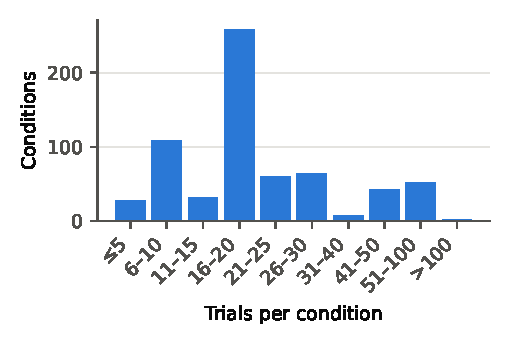
\includegraphics[width=0.48\linewidth]{fig_n.pdf}\hfill
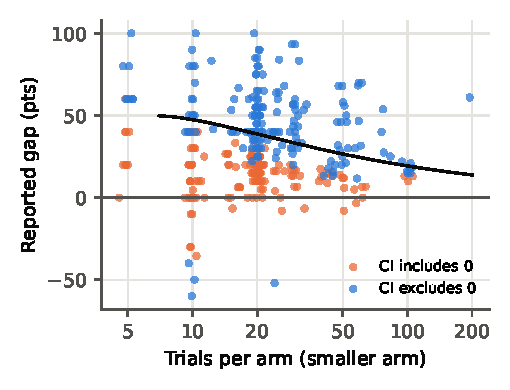
\includegraphics[width=0.48\linewidth]{fig_gap.pdf}
\caption{\textbf{Left:} trials per evaluated condition (\AuditConditions{} conditions, \AuditIncluded{} papers). \textbf{Right:} reported gap between the proposed method and its comparator against the number of trials in the smaller arm, for the \AuditPrimaryRows{} primary binary comparisons (log scale, small horizontal jitter). Blue: Newcombe 95\% interval excludes zero; orange: it does not. The black line is the gap an equal-arm study can detect with 80\% power when the comparator succeeds 50\% of the time.}
\label{fig:n}
\end{figure}

\begin{table}[t]
\centering
\caption{Reporting practice in the \AuditIncluded{} included papers (real-robot results).}
\label{tab:reporting}
\begin{tabular}{@{}lr@{}}
\toprule
Item reported & Share of papers\\ \midrule
Explicit success criterion & \AuditRepSuccessDef\\
Randomised or matched initial conditions & \AuditRepRandInit\\
Interval or error bars on success rate & \AuditRepCI\\
Number of training seeds & \AuditRepSeeds\\
Any significance test & \AuditRepTest\\
\bottomrule
\end{tabular}
\end{table}

\subsection{How many comparisons are resolved? (A3)}
Table~\ref{tab:compare} gives the main result. The proposed method scored higher than its comparator in \AuditSharePBetter{} of the \AuditPrimaryRows{} primary comparisons, with a median gap of \AuditMedianDiff{} points. The Newcombe interval for the difference excluded zero in \AuditShareCIExcl{} of comparisons: \AuditShareBCIExcl{} against the strongest baseline and \AuditShareACIExcl{} against the no-signal ablation. The Fisher test was significant in \AuditShareFisherSig{}; Boschloo's more powerful unconditional test in \AuditShareBoschlooSig{}, with the two disagreeing on \AuditFisherBoschlooDisagree{} comparisons. Using all \AuditBinaryRows{} rows instead of the primary set gives \AuditSensAllRowsCIExcl{} resolved, and excluding rows whose counts were reconstructed from ambiguous percentages gives \AuditSensNoAmbCIExcl{}.

Figure~\ref{fig:n} (right) shows why. Most comparisons sit at 10--25 trials per arm, where a gap must be 35--50 points to be detected reliably. Many reported gaps of 20--40 points fall below that line: large enough to be interesting, too small to be distinguished from noise at that sample size.

\begin{table}[t]
\centering
\caption{Statistical resolution of the primary binary comparisons. ``Resolved'' = Newcombe 95\% interval for the difference excludes zero. Required $n$: trials per arm for 80\% power at the observed rates (arcsine approximation). MDD: minimum detectable improvement over the observed comparator rate at the reported $n$, 80\% power.}
\label{tab:compare}
\begin{tabular}{@{}lrrr@{}}
\toprule
 & All & vs strongest baseline (B) & vs no-signal ablation (A)\\ \midrule
Comparisons & \AuditPrimaryRows & \AuditPrimaryRowsB & \AuditPrimaryRowsA\\
Proposed method higher & \AuditSharePBetter & \AuditShareBPBetter & \AuditShareAPBetter\\
Median reported gap (pts) & \AuditMedianDiff & \AuditMedianDiffB & \AuditMedianDiffA\\
Resolved (CI excludes 0) & \AuditShareCIExcl & \AuditShareBCIExcl & \AuditShareACIExcl\\
Fisher $p<0.05$ & \AuditShareFisherSig & \AuditShareBFisherSig & \AuditShareAFisherSig\\
Boschloo $p<0.05$ & \AuditShareBoschlooSig & \AuditShareBBoschlooSig & \AuditShareABoschlooSig\\
Median required $n$ per arm & \AuditMedianReqN & \AuditMedianReqNB & \AuditMedianReqNA\\
Reported $n$ $\ge$ required $n$ & \AuditShareAdequateN & \AuditShareAdequateNB & \AuditShareAdequateNA\\
Median MDD (pts) & \AuditMedianMDD & \AuditMedianMDDB & \AuditMedianMDDA\\
\bottomrule
\end{tabular}
\end{table}

\subsection{Paper-level resolution (A4)}
Papers usually make several comparisons, and their claims rest on the pattern. Without correction, \AuditPapersUnadjAtLeastOne{} of the \AuditPapersWithComparisons{} papers with binary comparisons had at least one significant comparison, \AuditPapersUnadjMajority{} had a majority, and \AuditPapersUnadjAll{} had all. After Holm correction within each paper these fell to \AuditPapersHolmAtLeastOne{}, \AuditPapersHolmMajority{} and \AuditPapersHolmAll{}. Against the strongest baseline alone, \AuditPapersBHolmAll{} of papers had every comparison resolved after correction; against the no-signal ablation, \AuditPapersAHolmAll{}. The claim that the force or touch signal itself is responsible for the gain therefore rests, in most papers, on at least one comparison that the data cannot yet distinguish from chance.

\subsection{How many trials would have been needed? (A5)}\label{sec:power}
At the observed rates, the median comparison needed \AuditMedianReqN{} trials per arm for 80\% power by the standard arcsine approximation (\AuditMedianReqNB{} against the strongest baseline), and only \AuditShareAdequateN{} of comparisons met that number. The arcsine formula, however, is optimistic in this literature. Many comparisons are lopsided (e.g.\ 18/20 vs 2/20, or 20/20 vs 12/20), and at the small $n$ it recommends for them the exact test has much less power than nominal: over the \AuditExactChecked{} comparisons we checked by full enumeration, the exact Fisher test had a mean power of \AuditExactPowerAtArcsineN{} at the arcsine $n$, and below 0.70 in \AuditShareExactPowerBelowSeventy{} of them. The exact required sample size was a median \AuditExactOverArcsineN{} times the arcsine value (median \AuditMedianExactReqN{} trials per arm), and only \AuditShareAdequateExactN{} of comparisons met it. Researchers planning evaluations should compute exact power for binomial comparisons rather than rely on the normal approximation, especially when one arm is expected near 0\% or 100\%.

\subsection{How often do equal methods look different? (A6)}
Table~\ref{tab:null} and Figure~\ref{fig:null} show the null simulation at $p=0.5$ (results at 0.3 and 0.7 are similar and released). With one task and 10 trials per arm, two equally good methods differ by at least 10 points \AuditNullTenOneFiveOne{} of the time; at 20 trials, \AuditNullTwentyOneFiveOne{}. Reporting the best of several variants raises these numbers: at 20 trials, the best of five variants shows a gain of at least 20 points \AuditNullTwentyOneFiveFiveTwenty{} of the time. Averaging over more tasks reduces the noise of the mean gain, but selection across variants largely undoes this: at 10 trials per arm, reporting the best of three variants over three tasks still shows a mean gain of 10 points or more \AuditNullTenThreeFiveThree{} of the time. Non-monotonicity at very small $n$ (5 vs 10 trials) is a discreteness effect: with 5 trials the smallest possible nonzero gap is 20 points.

\begin{figure}[t]
\centering
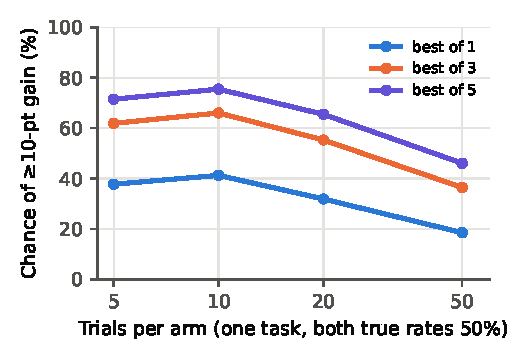
\includegraphics[width=0.5\linewidth]{fig_null.pdf}
\caption{Chance that a method with no true advantage shows an apparent gain of at least 10 points over a baseline, both with true success rate 50\%, one task, when the best of $m$ variants of the method is reported (200{,}000 simulated studies per point).}
\label{fig:null}
\end{figure}

\begin{table}[t]
\centering
\caption{Null simulation (A6), true rate 0.5 for both methods: probability (\%) that the reported mean gain over $k$ tasks, taking the best of $m$ variants, is at least 10 or 20 points.}
\label{tab:null}
\begin{tabular}{@{}rrrrrrrr@{}}
\toprule
 & & \multicolumn{3}{c}{$\Pr(\text{gain}\ge 10)$} & \multicolumn{3}{c}{$\Pr(\text{gain}\ge 20)$}\\
\cmidrule(lr){3-5}\cmidrule(l){6-8}
$n$ & $k$ & $m{=}1$ & $m{=}3$ & $m{=}5$ & $m{=}1$ & $m{=}3$ & $m{=}5$\\ \midrule
5 & 1 & 38 & 62 & 71 & 38 & 62 & 71\\
5 & 3 & 29 & 52 & 62 & 18 & 36 & 45\\
5 & 5 & 24 & 45 & 55 & 10 & 22 & 30\\
\addlinespace
10 & 1 & 41 & 66 & 75 & 25 & 46 & 56\\
10 & 3 & 26 & 47 & 58 & 8 & 18 & 24\\
10 & 5 & 18 & 36 & 46 & 3 & 7 & 10\\
\addlinespace
20 & 1 & 32 & 55 & 65 & 13 & 28 & 36\\
20 & 3 & 16 & 32 & 41 & 2 & 5 & 7\\
20 & 5 & 9 & 20 & 27 & 0 & 1 & 1\\
\addlinespace
50 & 1 & 18 & 36 & 46 & 3 & 7 & 10\\
50 & 3 & 5 & 11 & 16 & 0 & 0 & 0\\
50 & 5 & 1 & 4 & 5 & 0 & 0 & 0\\
\bottomrule
\end{tabular}

\end{table}

\subsection{What would a sequential test cost? (A7)}
Table~\ref{tab:sprt} shows a simple sequential test that alternates trials of the two methods and stops when the evidence crosses a boundary. Designed to detect 70\% vs 50\%, it needed on average \AuditSPRTPairsSeventy{} trials per method when that was the truth, against \AuditFixedNSeventy{} for a fixed-sample exact test with the same error rates, and stopped after \AuditSPRTPairsNull{} trials on average when the methods were equal. Much larger true gaps, which several papers report, are confirmed in fewer trials still. Near-optimal sequential tests for robot policy comparison, with proper handling of composite hypotheses and a maximum budget, are available~\cite{snyder2025step,snyder2026nscore}; the SPRT here is only an illustration of the order of magnitude.

\begin{table}[t]
\centering
\caption{Wald SPRT on discordant pairs, designed for $p_X=0.5$ vs $p_P=0.7$ (one-sided $\alpha=0.025$, power 0.8, at most 500 pairs; 20{,}000 replicates). A fixed-sample two-sided Fisher test with 80\% power at 0.5 vs 0.7 needs \AuditFixedNSeventy{} trials per arm.}
\label{tab:sprt}
\begin{tabular}{@{}lrrr@{}}
\toprule
True rates ($p_X$, $p_P$) & Mean trials per arm & $\Pr$(decide for P) & $\Pr$(no decision)\\ \midrule
(0.5, 0.5) & 39 & 0.024 & 0.000\\
(0.5, 0.6) & 76 & 0.321 & 0.001\\
(0.5, 0.7) & 67 & 0.844 & 0.000\\
(0.5, 0.8) & 42 & 0.983 & 0.000\\
(0.5, 0.9) & 29 & 1.000 & 0.000\\
\bottomrule
\end{tabular}

\end{table}

\section{Discussion}\label{sec:discussion}
\textbf{What the numbers mean.} The pattern is consistent. Proposed methods almost always score higher, and the gaps are often large, but the typical evaluation of 10--25 trials per arm can only distinguish gaps of 35--50 points from noise. About half of individual comparisons, and a minority of papers taken as a whole, are statistically resolved. Low power also means that the gaps which do pass a significance filter are likely to overstate the true effect~\cite{button2013,gelman2014}, and our null simulation shows that common reporting choices, such as reporting the best variant or configuration, make 10--20 point gains easy to obtain by chance. None of this implies that the force or touch signals do not help; the direction of the evidence is clearly positive. It implies that the size of the benefit, and which design choices produce it, are much less certain than the tables suggest.

\textbf{Why it happens.} Real-robot trials are expensive, and the incentive is to spend them across many tasks and baselines rather than on many trials per comparison. A paper with six tasks, four baselines and an ablation at 20 trials each runs 720 trials, a substantial effort, yet each cell is underpowered. Statistical reporting is also not expected by reviewers in this area. The fix is therefore partly cultural and partly a matter of allocating the same effort differently.

\textbf{A short checklist.} Based on the audit, we suggest the following for real-robot comparisons, most of which cost no extra trials:
\begin{enumerate}[leftmargin=*,itemsep=1pt]
\item Report successes \emph{and} trials ($k/n$) for every cell, not only percentages.
\item Give a 95\% interval for each rate (Wilson) and for each headline difference (Newcombe).
\item Pre-specify one or two headline comparisons per paper, test them (Fisher or Boschloo), and correct for multiplicity when several comparisons support one claim.
\item Plan $n$ with exact binomial power for the gap you expect, not the normal approximation; when the budget is fixed, report the minimum detectable gap.
\item Prefer fewer, better-powered comparisons for the central claim; pool clearly related tasks only when the claim is about the pool.
\item Use a sequential test when trials are expensive and gaps may be large~\cite{snyder2025step}.
\item State how the reported variant or configuration was chosen, and report the others.
\item Say ``not resolved at this sample size'' rather than ``outperforms'' when the interval includes zero.
\end{enumerate}

\section{Limitations}
\textbf{Sample.} The audit covers papers retrieved by six fixed queries from one search interface that ranks recent work first; it is a snapshot of 2026 work, not a census, and may over-represent prominent or recent papers. Most are preprints, and published versions may differ.

\textbf{Extraction.} Both extractions were done by the same kind of language-model assistant under the author's supervision; although the second was blinded to values and decisions, the two may share systematic errors, and verifiers received the first extraction's task and comparator list, so omissions in that list were only partly checked (verifiers were asked to report missing comparisons). Coding rules required judgment (which baseline is eligible as ``strongest'', what counts as a no-signal ablation), and we made several of these rules explicit only during extraction; all are logged with dates, and none was introduced after analysis. Reconstructing counts from percentages introduces small errors, which the sensitivity analysis addresses.

\textbf{Statistics.} We treat trials as independent Bernoulli outcomes and the two arms as independent. Many papers use matched initial conditions, for which paired analyses would be more powerful, and some pool trials across training seeds, which ignores clustering. We test each comparison on its own, whereas papers often argue from consistency across tasks; a hierarchical model would use that information, at the cost of further assumptions. Partial-credit outcomes were excluded from tests.

\textbf{Scope of conclusions.} Unresolved comparisons are not evidence of no effect. We did not attempt to judge any paper's contribution, and the per-paper data are released for checking, not ranking.

\section{Conclusion}
In 2026 work on force-, tactile- and current-aware manipulation, real-robot claims rest on a median of \AuditMedianN{} trials per condition, rarely with any statement of uncertainty. Under standard binomial statistics about half of individual comparisons, and a small minority of papers as a whole, are resolved, and the typical study can only detect gaps of 35 points or more. The methods may well be as good as reported; the evaluations mostly cannot tell. Reporting $k/n$ with intervals, testing a few pre-specified comparisons with exact methods, and allocating trials to the central claim, or using sequential tests, would make the same effort far more informative.

\section*{Data and code availability}
The frozen protocol with all dated deviations, per-paper extraction records with sources and notes, the blinded verification packets and outputs, the adjudication log, the analysis code with unit tests, and all generated tables are released at [repository URL to be added]. Every number in this paper is read from files generated by the released scripts.

\section*{Acknowledgements and disclosure}
Extraction, verification and analysis code were produced with the assistance of an AI model (Claude, Anthropic) under the author's direction; the author defined the protocol, adjudicated all discrepancies against the source papers and takes responsibility for the content.

\begin{thebibliography}{99}\small
\bibitem{agarwal2021} R.~Agarwal, M.~Schwarzer, P.~S. Castro, A.~C. Courville, and M.~G. Bellemare. Deep reinforcement learning at the edge of the statistical precipice. In \emph{Advances in Neural Information Processing Systems}, vol.~34, 2021.
\bibitem{aidoo2026a} C.~Aidoo. Gravity pivoting from motor current: calibration-free angle estimation and the sensing budget it requires. engrXiv preprint, doi:10.31224/8492, 2026.
\bibitem{boschloo1970} R.~D. Boschloo. Raised conditional level of significance for the $2\times2$-table when testing the equality of two probabilities. \emph{Statistica Neerlandica}, 24(1):1--9, 1970.
\bibitem{button2013} K.~S. Button, J.~P.~A. Ioannidis, C.~Mokrysz, B.~A. Nosek, J.~Flint, E.~S.~J. Robinson, and M.~R. Munaf\`o. Power failure: why small sample size undermines the reliability of neuroscience. \emph{Nature Reviews Neuroscience}, 14(5):365--376, 2013.
\bibitem{cohen1988} J.~Cohen. \emph{Statistical Power Analysis for the Behavioral Sciences}, 2nd ed. Lawrence Erlbaum, 1988.
\bibitem{colas2018} C.~Colas, O.~Sigaud, and P.-Y. Oudeyer. How many random seeds? Statistical power analysis in deep reinforcement learning experiments. arXiv:1806.08295, 2018.
\bibitem{fisher1922} R.~A. Fisher. On the interpretation of $\chi^2$ from contingency tables, and the calculation of P. \emph{Journal of the Royal Statistical Society}, 85(1):87--94, 1922.
\bibitem{gelman2014} A.~Gelman and J.~Carlin. Beyond power calculations: assessing Type S (sign) and Type M (magnitude) errors. \emph{Perspectives on Psychological Science}, 9(6):641--651, 2014.
\bibitem{henderson2018} P.~Henderson, R.~Islam, P.~Bachman, J.~Pineau, D.~Precup, and D.~Meger. Deep reinforcement learning that matters. In \emph{Proceedings of the AAAI Conference on Artificial Intelligence}, 32(1), 2018.
\bibitem{holm1979} S.~Holm. A simple sequentially rejective multiple test procedure. \emph{Scandinavian Journal of Statistics}, 6(2):65--70, 1979.
\bibitem{ioannidis2005} J.~P.~A. Ioannidis. Why most published research findings are false. \emph{PLoS Medicine}, 2(8):e124, 2005.
\bibitem{kressgazit2024} H.~Kress-Gazit, K.~Hashimoto, N.~Kuppuswamy, P.~Shah, P.~Horgan, G.~Richardson, S.~Feng, and B.~Burchfiel. Robot learning as an empirical science: best practices for policy evaluation. arXiv:2409.09491, 2024.
\bibitem{newcombe1998} R.~G. Newcombe. Interval estimation for the difference between independent proportions: comparison of eleven methods. \emph{Statistics in Medicine}, 17(8):873--890, 1998.
\bibitem{scipy2020} P.~Virtanen et al. SciPy 1.0: fundamental algorithms for scientific computing in Python. \emph{Nature Methods}, 17:261--272, 2020.
\bibitem{snyder2025step} D.~Snyder, A.~J. Hancock, A.~Badithela, E.~Dixon, P.~Miller, R.~A. Ambrus, A.~Majumdar, M.~Itkina, and H.~Nishimura. Is your imitation learning policy better than mine? Policy comparison with near-optimal stopping. arXiv:2503.10966, 2025.
\bibitem{snyder2026nscore} D.~Snyder, A.~Badithela, N.~Matni, G.~Pappas, A.~Majumdar, M.~Itkina, and H.~Nishimura. Beyond binary success: sample-efficient and statistically rigorous robot policy comparison. arXiv:2603.13616, 2026.
\bibitem{wald1945} A.~Wald. Sequential tests of statistical hypotheses. \emph{The Annals of Mathematical Statistics}, 16(2):117--186, 1945.
\bibitem{wilson1927} E.~B. Wilson. Probable inference, the law of succession, and statistical inference. \emph{Journal of the American Statistical Association}, 22(158):209--212, 1927.
\end{thebibliography}

\appendix
\section{Protocol deviations}\label{app:deviations}
All deviations were committed to the repository, with timestamps, before they were applied; none was made after any analysis had been run on the corresponding data. In brief:
\textbf{D1} narrowed the window to 2026-01-01 -- 2026-09-30 because the search tool returns mostly recent work.
\textbf{D2} (a) excluded partial-credit outcomes from binomial tests; (b) defined kind A as the proposed method with the signal removed.
\textbf{D3} kept eligible papers with no stated trial counts in the reporting statistics.
\textbf{D4} counted camera-measured contact deformation, and RGB-generated tactile signals consumed through a tactile channel, as tactile.
\textbf{D5} restricted kind B to external or author-built baselines.
\textbf{D6} required the signal to be an input at deployment.
\textbf{D7} fixed analysis details before the first run: primary-row selection, Holm families, the reading of ``best of $m$'', exact power by enumeration, and the sequential-test design.
The full text is in the released protocol.

\section{Screened papers}
\begin{longtable}{@{}llrrrl@{}}
\caption{All screened papers. Binary = primary binary comparisons; resolved = Fisher $p<0.05$ after Holm correction within the paper. Per-row data, sources and coder notes are in the released data.}\label{tab:papers}\\
\toprule arXiv ID & Signal & Binary & Resolved & Median $n$ & Status \\ \midrule \endfirsthead
\toprule arXiv ID & Signal & Binary & Resolved & Median $n$ & Status \\ \midrule \endhead
\bottomrule \endfoot
2502.17432 & force & -- & -- & -- & excluded: date (D1) \\
2508.07118 & tactile & -- & -- & -- & excluded: date (D1) \\
2602.22088 & force & 16 & 1 & 10 & included \\
2603.04531 & tactile & -- & -- & -- & excluded: I2 \\
2603.05687 & tactile & 2 & 0 & 15 & included \\
2603.08342 & force & 5 & 0 & 20 & included \\
2603.13869 & tactile & -- & -- & -- & excluded: I3 \\
2605.28412 & mixed & -- & -- & -- & excluded: I1 \\
2606.04825 & tactile & 16 & 1 & 10 & included \\
2606.06281 & tactile & 10 & 5 & 20 & included \\
2606.08555 & force & 8 & 1 & 20 & included \\
2606.09337 & tactile & 4 & 0 & 30 & included \\
2606.10818 & torque & 4 & 2 & 25 & included \\
2606.11184 & mixed & 4 & 2 & 20 & included \\
2606.11767 & tactile & 0 & 0 & 100 & included \\
2606.12406 & current & 0 & 0 & 20 & included \\
2606.13232 & tactile & 0 & 0 & 25 & included \\
2606.14218 & torque & 8 & 2 & 20 & included \\
2606.17055 & tactile & 0 & 0 & 16 & included \\
2606.24450 & mixed & -- & -- & -- & excluded: I2 \\
2606.30988 & force & 3 & 0 & 15 & included \\
2607.02503 & tactile & 6 & 0 & 20 & included \\
2607.03387 & tactile & 10 & 0 & 25 & included \\
2607.03529 & current & 5 & 2 & 52 & included \\
2607.03723 & tactile & 8 & 8 & 20 & included \\
2607.07287 & tactile & 12 & 1 & 100 & included \\
2607.08575 & none & -- & -- & -- & excluded: I1 \\
2607.11734 & current & 2 & 0 & 40 & included \\
2607.14236 & force & 1 & 1 & 30 & included \\
2607.14578 & current & 6 & 2 & 20 & included \\
2607.18231 & force & 6 & 2 & 18 & included \\
2607.20683 & tactile & 8 & 0 & 20 & included \\
2607.20912 & force & 2 & 2 & 20 & included \\
2607.22530 & tactile & 8 & 4 & 50 & included \\
2608.01102 & tactile & 9 & 0 & 20 & included \\
2608.01733 & tactile & -- & -- & -- & excluded: I2 \\
2608.01824 & tactile & 1 & 0 & 20 & included \\
2608.07558 & mixed & -- & -- & -- & excluded: survey \\
2608.15009 & force & 10 & 1 & 45 & included \\
2608.15560 & tactile & 4 & 0 & 11 & included \\
2608.24603 & none & -- & -- & -- & excluded: I1 \\
2608.25798 & tactile & 6 & 0 & 16 & included \\
2608.25872 & tactile & 14 & 0 & 10 & included \\
2609.02020 & torque & -- & -- & -- & excluded: I2 \\
2609.03889 & torque & 6 & 6 & 25 & included \\
2609.05832 & force & 0 & 0 & 25 & included \\
2609.07002 & tactile & 5 & 2 & 200 & included \\
2609.07747 & tactile & 1 & 1 & 30 & included \\
2609.12549 & tactile & 6 & 2 & 20 & included \\
2609.13779 & torque & -- & -- & -- & excluded: I2 \\
2609.14156 & tactile & 8 & 2 & 30 & included \\
2609.15012 & force & 0 & 0 & 50 & included \\
2609.15726 & tactile & -- & -- & -- & excluded: I2 (sim.) \\
2609.15921 & tactile & 4 & 3 & 30 & included \\
2609.16437 & tactile & -- & -- & -- & excluded: I2 \\
2609.16504 & tactile & 11 & 0 & 10 & included \\
2609.16586 & none & -- & -- & -- & excluded: I1 \\
2609.18164 & torque & -- & -- & -- & excluded: I2 (sim.) \\
2609.18165 & tactile & -- & -- & -- & excluded: hardware only \\
2609.18242 & torque & 12 & 1 & 30 & included \\
2609.18497 & force & 12 & 5 & 30 & included \\
2609.19137 & force & 8 & 2 & 10 & included \\
2609.20649 & tactile & 0 & 0 & 10 & included \\
2609.20980 & tactile & 10 & 3 & 80 & included \\
2609.21369 & none & -- & -- & -- & excluded: I1 \\
2609.22840 & force & 3 & 3 & 30 & included \\
2609.22895 & none & -- & -- & -- & excluded: I1 \\
2609.23614 & force & -- & -- & -- & excluded: I1 \\
2609.23800 & mixed & 3 & 3 & 50 & included \\
2609.23888 & current & 3 & 2 & 20 & included \\
2609.23968 & force & -- & -- & -- & excluded: I2 \\
2609.24976 & tactile & 4 & 2 & 20 & included \\
2609.25785 & force & 3 & 3 & 20 & included \\
2609.27381 & current & -- & -- & -- & excluded: I2 \\
2609.29017 & current & 0 & 0 & 30 & included \\
2609.29822 & tactile & 8 & 4 & 60 & included \\
2609.30969 & tactile & 1 & 0 & 20 & included \\
2609.31924 & force & 3 & 3 & 20 & included \\
2609.33882 & tactile & -- & -- & -- & excluded: I1 \\
2609.34006 & tactile & 1 & 1 & 20 & included \\
2609.34182 & tactile & 0 & 0 & 10 & included \\
2609.34286 & tactile & -- & -- & -- & excluded: I2 \\
2609.34400 & force & -- & -- & -- & excluded: I2 \\
2609.36596 & tactile+torque & 10 & 7 & 20 & included \\
2609.36785 & tactile & -- & -- & -- & excluded: I1 (D6) \\
2609.37433 & force & 6 & 3 & 25 & included \\
2609.37552 & force & 5 & 3 & 50 & included \\
2609.39017 & tactile & -- & -- & -- & excluded: I3 \\
2610.00638 & tactile & 10 & 0 & 20 & included \\
\end{longtable}


\end{document}
